\documentclass[a4paper]{article}

\input{style/ch_xelatex.tex}


\lstset{frame=, basicstyle={\footnotesize\ttfamily}}



\graphicspath{ {images/} }
\usepackage{ctex}
\usepackage{amsmath}
\usepackage{geometry}

\geometry{a4paper,left=3.5cm,right=3.5cm,top=4cm,bottom=4cm}


%-----------------------------------------BEGIN DOC----------------------------------------

\begin{document}
\renewcommand{\contentsname}{目\ 录}
\renewcommand{\appendixname}{附录}
\renewcommand{\appendixpagename}{附录}
\renewcommand{\refname}{参考文献} 
\renewcommand{\figurename}{图}
\renewcommand{\tablename}{表}
\renewcommand{\today}{\number\year 年 \number\month 月 \number\day 日}


\title{{\Huge EE229 实验报告{\large\linebreak\\}}{\Large 实验一 \ 图像处理基础\linebreak\linebreak}}
%please write your name, Student #, and Class # in Authors, student ID, and class # respectively
\author{\\姓\ \ \ \ \ \ \ 名:洪峰\  \ \ \  \ \ \ \ \ \ \ \ \ \ \ \ \ \ \ \ \ \ \ \ \ \ \ \ \ \\
学\ \ \ \ \ \ \ 号:\ 517021910418\ \ \ \ \ \ \ \ \ \ \ \ \ \ \ \ \ \\ 
专\ \ \ \ \ \ \ 业:信息工程 \ \ \  \ \ \ \    \ \ \ \ \ \ \ \ \ \ \ \ \ \ \ \   \\
学\ \ \ \ \  \  \ 院:电子信息与电气工程学院\\
指导老师:周军 \ \ \ \ \ \ \ \ \ \ \ \ \ \ \ \  \ \ \ \ \ \ \ \ \ \ \ \ \ \\\\\\\\\\
 {\LARGE EE229 数字图像处理}\\\\\\\\\\\\\\\\\\
上海交通大学\\
}

\date{\today}
\maketitle
\newpage

%-----------------------------------------ABSTRACT-------------------------------------
%\begin{center}
%{\Large\bf{摘\ 要\\}}
%\end{center}
%请在这里输入摘要内容.
%\newpage
%-----------------------------------------ABSTRACT-------------------------------------

%\begin{center}
%\Large\bf{版\ 权\ 声\ 明\\}}
%\end{center}
%该文件受《中华人名共和国著作权法》的保护。ERCESI实验室保留拒绝授权违法复制该文件的权利。任何收存和保管本文件各种版本的单位和个人,未经ERCESI实验室(西北工业大学)同意,不得将本文档转借他人,亦不得随意复制、抄录、拍照或以任何方式传播。 否则,引起有碍著作权之问题,将可能承担法律责任。\newpage
%-----------------------------------------CONTENT-------------------------------------
\begin{center}
\tableofcontents\label{c}
\end{center}
\newpage

%------------------------------------------TEXT--------------------------------------------

%----------------------------------------
%实验任务-----------------------------------------

\section{实验任务} \label{overview}%------------------------------
\subsection{任务一}

\begin{itemize}
	\item 输入一张灰度图(rose.tif),对其进行2倍,4倍,8倍,16倍,32倍的下采样,并对下采样的图像用双线性插值进行放大,计算对应的$PSNR$值;
    \item 要求:下采样、双线性插值、$PSNR$计算都要自己编程实现,并与matlab自带的库函数处理结果进行对比,分析结果。

\end{itemize}
\subsection{任务二}

\begin{itemize}
	\item 输入一张灰度图(rose.tif),对其进行2倍,4倍,8倍,16倍,32倍的下采样,并对下采样的图像用双线性插值进行放大,计算对应的$PSNR$值;
    \item 要求:下采样、双线性插值、$PSNR$计算都要自己编程实现,并与matlab自带的库函数处理结果进行对比,分析结果。

\end{itemize}
\subsection{任务三}

\begin{itemize}
	\item 输入一张灰度图(rose.tif),对其进行2倍,4倍,8倍,16倍,32倍的下采样,并对下采样的图像用双线性插值进行放大,计算对应的$PSNR$值;
    \item 要求:下采样、双线性插值、$PSNR$计算都要自己编程实现,并与matlab自带的库函数处理结果进行对比,分析结果。

\end{itemize}

%------------------------------------实验原理--------------------------------------

\newpage
%------------------------------
\section{实验原理}\label{sub:ptx}
\subsection{图像缩放}
在计算机图形学和数字成像中,图像 缩放是指调整数字图像的大小。缩放矢量图时,可以使用几何变换来缩放组成该图像的图形基元,而不会降低图像质量。缩放位图时,必须生成像素数更高或更低的新图像。在减少像素数量(按比例缩小,即下采样)的情况下,这通常会导致可见的质量损失。从数字信号处理的角度来看,位图的缩放是采样率转换的二维示例,即离散信号从采样率(在这种情况下为本地采样率)到另一个采样率的转换。

对于一幅图像I尺寸为$M\cdot N$,对其进行$s$倍下采样,即得到$(\frac{M}{s})\cdot (\frac{N}{s})$尺寸的分辨率图像。如果考虑的是矩阵形式的图像,就是把原始图像$s\cdot s$窗口内的图像变成一个像素,相当于池化的操作。
图像放大(即上采样)几乎都是采用内插值方法,即在原有图像像素的基础上在像素点之间采用合适的插值算法插入新的元素。
\subsection{双线形插值}
在数学上,双线性插值是有两个变量的插值函数的线性插值扩展,其核心思想是在两个方向分别进行一次线性插值。

\begin{figure}[h]
\centering
\includegraphics[scale=0.45]{images/sxx.pdf}
\caption{双线性插值示意图}
\label{fig:sxx}
\end{figure}

假如我们想得到未知函数$f$ 在点$ P = (x, y)$ 的值,已知函数$ f$ 在 $Q_{11} = (x_1, y_1)$、$Q_{12} = (x_1, y_2)$,$ Q_{21} = (x_2, y_1)$ 以及 $Q_{22} = (x_2, y_2)$ 四个点的值。

如图\ref{fig:sxx}所示,首先在$ x$ 方向进行线性插值,得到
\[f(R_1) \approx \dfrac{x_2-x}{x_2-x_1}f(Q_{11})+\dfrac{x-x_1}{x_2-x_1}fQ_{21})\]

然后在 y 方向进行线性插值,得到
\[f(R_2) \approx \dfrac{x_2-x}{x_2-x_1}f(Q_{12})+\dfrac{x-x_1}{x_2-x_1}fQ_{22})\]

这样就得到所要的结果 $f(x, y)$。
\begin{equation*}
\begin{split}
f(x,y) \approx  \dfrac{f(Q_{11})}{(x_2-x_1)(y_2-y_1)}(x_2-x)(y_2-y)+\dfrac{f(Q_{21})}{(x_2-x_1)(y_2-y_1)}(x-x_1)(y_2-y) \\
 +\dfrac{f(Q_{12})}{(x_2-x_1)(y_2-y_1)}(x_2-x)(y-y_1)+\dfrac{f(Q_{22})}{(x_2-x_1)(y_2-y_1)}(x-x_1)(y-y_1)
\end{split}
\end{equation*}

\subsection{RGB颜色空间}
RGB颜色空间以R(Red:红)、G(Green:绿)、B(Blue:蓝)三种基本色为基础,进行不同程度的叠加,产生丰富而广泛的颜色,所以俗称三基色模式。在大自然中有无穷多种不同的颜色,而人眼只能分辨有限种不同的颜色,RGB模式可表示一千六百多万种不同的颜色,在人眼看来它非常接近大自然的颜色,故又称为自然色彩模式。红绿蓝代表可见光谱中的三种基本颜色或称为三原色,每一种颜色按其亮度的不同分为256个等级。当色光三原色重叠时,由于不同的混色比例能产生各种中间色。

将R、G、B三个通道作为笛卡尔坐标系中的X、Y、Z轴,就得到了一种对于颜色的空间描述,如图\ref{fig:rgb}。



\subsection{HSI颜色空间}
\subsubsection{HSI空间简介}
HSI〔Hue-Saturation-Intensity(Lightness),HSI或HSL〕颜色模型用H、S、I三参数描述颜色特性,其中H定义颜色的波长,称为色调;S表示颜色的深浅程度,称为饱和度;I表示强度或亮度。

\begin{figure}[H]
\centering
\includegraphics[scale=0.33]{images/rgb.pdf}
\caption{RGB颜色空间}
\label{fig:rgb}
\end{figure}

颜色模型从人的视觉系统出发,用H,S,I三个参数来描述色彩,它反映了人的视觉系统感知彩色的方式,这种彩色描述对人来说是直观的、自然的。色调H 是描述纯色的属性(如红色、黄色等);饱和度S 表示的是一种纯色被白光稀释的程度的度量;强度I 是一个主观的描述,是人对彩色感觉的关键参数,实际上它是不可能测量的。HSI模型可从彩色图像中携带的彩色信息(色调和饱和度)里消去强度分量的影响,因而使得该模型在开发基于彩色描述的图像处理算法中非常有用。



\begin{figure}[H]
\centering
\includegraphics[scale=0.32]{images/hsi.pdf}
\caption{HSI颜色空间}
\label{fig:hsi}
\end{figure}

HSI颜色空间可以用一个圆锥空间模型来描述,如图\ref{fig:hsi}。用这种描述HSI色彩空间的圆锥模型相当复杂,但确能把色调、亮度和色饱和度的变化情形表现得很清楚。

\subsubsection{RGB转换为HSI}
现有一个RGB空间图像,通过以下式子得到HSI图像。

色调H:
\begin{equation*}  
H=\frac{1}{2\pi}
\left\{  
             \begin{array}{lr}
             \theta, & B\leq G   \\  
             2\pi-\theta, & B>G
             
             \end{array}  
\right.  
where \ \theta=\arccos \bigg (  \dfrac{0.5\times(2R-G-B)}{\sqrt{(R-G)^2+(R-G)(G-B)}} \bigg )
\end{equation*}  

饱和度S:
\begin{equation*}  
H=1-\dfrac{3min(R,G,B)}{R+G+B}
\end{equation*}  

强度分量I:
\begin{equation*}  
I=\dfrac{R+G+B}{3}
\end{equation*} 

\subsubsection{HSI转换为RGB}
HSI给出的区间是$[0,1]$,现在我们在相同的值域中找出对应的RGB值。首先将色调值H调回$[0^\circ,360^\circ]$,并进一步调整至区间$[0^\circ,120^\circ]$(通过减去$120^\circ$的整数倍实现)。进一步得出图片的RGB值:
\begin{equation*}%加*表示不对公式编号
B=I(1-S)
\end{equation*}
\begin{equation*}%加*表示不对公式编号
R=I\bigg [ 1+\frac{S\cdot cosH}{cod(60^\circ -H)} \bigg ]
\end{equation*}

\begin{equation*}%加*表示不对公式编号
G=3I-(R+B)
\end{equation*}

\subsection{YUV颜色空间}
\subsubsection{YUV空间简介}
YUV(亦称YCrCb)是被欧洲电视系统所采用的一种颜色编码方法。在现代彩色电视系统中,通常采用三管彩色摄像机或彩色CCD摄影机进行取像,然后把取得的彩色图像信号经分色、分别放大校正后得到RGB,再经过矩阵变换电路得到亮度信号Y和两个色差信号R-Y(即U)、B-Y(即V),最后发送端将亮度和两个色差总共三个信号分别进行编码,用同一信道发送出去。这种色彩的表示方法就是所谓的YUV色彩空间表示。采用YUV色彩空间的重要性是它的亮度信号Y和色度信号U、V是分离的。如果只有Y信号分量而没有U、V信号分量,那么这样表示的图像就是黑白灰度图像。彩色电视采用YUV空间正是为了用亮度信号Y解决彩色电视机与黑白电视机的兼容问题,使黑白电视机也能接收彩色电视信号。

YUV主要用于优化彩色视频信号的传输,使其向后相容老式黑白电视。与RGB视频信号传输相比,它最大的优点在于只需占用极少的频宽(RGB要求三个独立的视频信号同时传输)。其中“Y”表示明亮度(Luminance或Luma),也就是灰阶值;而“U”和“V” 表示的则是色度(Chrominance或Chroma),作用是描述影像色彩及饱和度,用于指定像素的颜色。“亮度”是透过RGB输入信号来建立的,方法是将RGB信号的特定部分叠加到一起。“色度”则定义了颜色的两个方面─色调与饱和度,分别用Cr和Cb来表示。其中,Cr反映了RGB输入信号红色部分与RGB信号亮度值之间的差异。而Cb反映的是RGB输入信号蓝色部分与RGB信号亮度值之同的差异。

\subsubsection{YUV空间与RGB空间的互相转换}
YUV颜色模型到RGB颜色模型的转换,应该对应两种方式,分别是模拟YUV与模拟RGB转换、数字YUV与数字RGB互相转换。不过因为标清、高清、以及超清幅面,YUV转RGB的权重值各不相同,需要将模拟信号和数字信号再做一次幅面划分。下面介绍几种常见的转换矩阵。
\begin{itemize}
	\item 模拟YUV与模拟RGB转换
	\begin{enumerate}
	    \item BT601(标清国际定义)\\
	    \begin{equation*}
	         \left(\begin{matrix}
                 Y \\Pb \\Pr\end{matrix}\right)
                 =
            \left(\begin{matrix}
                 0.299 & 0.587 & 0.114 \\-0.169 & -0.331 & 0.500 \\0.500 & -0.439 & -0.081 \end{matrix}\right)
            \left(\begin{matrix}
                 R \\G \\B
            \end{matrix}\right)
	    \end{equation*}
	    \begin{equation*}
	         \left(\begin{matrix}
                 R \\G \\B\end{matrix}\right)
                 =
            \left(\begin{matrix}
                 1 & 0 & 1.402 \\1 & -0.344 & -0.792 \\1 & 1.772 & 0 \end{matrix}\right)
            \left(\begin{matrix}
                Y \\Pb \\Pr
            \end{matrix}\right)
	    \end{equation*}
	    \item BT709(高清) \\
	    \begin{equation*}
	         \left(\begin{matrix}
                 Y \\Pb \\Pr\end{matrix}\right)
                 =
            \left(\begin{matrix}
                 0.231 & 0.715 & 0.072 \\-0.115 & -0.385 & 0.500 \\0.500 & -0.454 & -0.046 \end{matrix}\right)
            \left(\begin{matrix}
                 R \\G \\B
            \end{matrix}\right)
	    \end{equation*}
	    \begin{equation*}
	         \left(\begin{matrix}
                 R \\G \\B\end{matrix}\right)
                 =
            \left(\begin{matrix}
                 1 & 0 & 1.402 \\1 & -0.344 & -0.792 \\1 & 1.772 & 0 \end{matrix}\right)
            \left(\begin{matrix}
                Y \\Pb \\Pr
            \end{matrix}\right)
	    \end{equation*}
	\end{enumerate}
    \item 数字YUV与数字RGB转换
    \begin{enumerate}
        \item BT601(标清国际定义) \\
	    \begin{equation*}
	         \left(\begin{matrix}
                 Y \\Cb \\Cr\end{matrix}\right)
                 =
                 \left(\begin{matrix}
                 16 \\128 \\128
            \end{matrix}\right)+
            \left(\begin{matrix}
                 0.257 & 0.504 & 0.098 \\-0.148 & -0.291 & 0.439 \\0.439 & -0.368 & -0.071 \end{matrix}\right)
            \left(\begin{matrix}
                 R \\G \\B
            \end{matrix}\right)
	    \end{equation*}
	    \begin{equation*}
	         \left(\begin{matrix}
                 R \\G \\B\end{matrix}\right)
                 =
            \left(\begin{matrix}
                 1.164 & 0 & 1.596 \\1.164 & -0.392 & -0.812 \\1.164 & 2.016 & 0 \end{matrix}\right)
            \left(\begin{matrix}
                Y-16 \\Cb-128 \\Cr-128
            \end{matrix}\right)
	    \end{equation*}
	    \item BT709(高清)
	    \begin{equation*}
	         \left(\begin{matrix}
                 Y \\Cb \\Cr\end{matrix}\right)
                 =
                 \left(\begin{matrix}
                 16 \\128 \\128
            \end{matrix}\right)+
            \left(\begin{matrix}
                 0.183 & 0.614 & 0.062 \\-0.101 & -0.339 & 0.439 \\0.439 & -0.399 & -0.040 \end{matrix}\right)
            \left(\begin{matrix}
                 R \\G \\B
            \end{matrix}\right)
	    \end{equation*}
	    \begin{equation*}
	         \left(\begin{matrix}
                 R \\G \\B\end{matrix}\right)
                 =
            \left(\begin{matrix}
                 1.164 & 0 & 1.792 \\1.164 & -0.213 & -0.534 \\1.164 & 2.114 & 0 \end{matrix}\right)
            \left(\begin{matrix}
                Y-16 \\Cb-128 \\Cr-128
            \end{matrix}\right)
	    \end{equation*}
    \end{enumerate}

\end{itemize}
\subsubsection{YUV采样格式}
YUV主流的采样方式有三种,YUV4:4:4,YUV4:2:2,YUV4:2:0,如图\ref{fig:yuv}所示。
\begin{itemize}
    \item \textbf{4:4:4采样}:每个Y分量对应一组UV分量
    \item \textbf{4:2:2采样}:每2个Y分量对应一组UV分量
    \item \textbf{4:2:0采样}:每4个Y分量对应一组UV分量
\end{itemize}
\begin{figure}[htbp]
    \centering
    \includegraphics[scale=0.43]{images/yuv.pdf}
    \caption{三种采样格式示意图}
    \label{fig:yuv}
\end{figure}

\subsection{峰值信噪比$PSNR$}
峰值信噪比(Peak signal-to-noise ratio,$PSNR$)是一个表示信号最大可能功率和影响它的表示精度的破坏性噪声功率的比值的工程术语。由于许多信号都有非常宽的动态范围,峰值信噪比常用对数分贝单位来表示。峰值信噪比经常用作图像压缩等领域中信号重建质量的测量方法,它常简单地通过均方误差(MSE)进行定义。

\subsubsection{$PSNR$计算}
两个$m\times n$单色图像$I$和$K$,如果一个为另外一个的噪声近似,那么它们的的均方误差定义为:
\begin{equation*}
    MSE=\frac{1}{MN}\sum_{i=0}^{M-1}\sum_{j=0}^{N-1}\left\|I(i,j)-K(i,j)\right\|^2
\end{equation*}

峰值信噪比$PSNR$定义为:
\begin{equation*}
PSNR=10lg\left( \frac{MAX_I^2}{MSE}\right)=20lg\left( \frac{MAX_I}{\sqrt{MSE} }\right)
\end{equation*}

其中,$MAX_I$是表示图像点颜色的最大数值,如果每个采样点用 8 位表示,那么就是 255。一般的,如果每个采样点用 B 位线性脉冲编码调制表示,那么 $MAX_I$ 就是$2^B-1$。

\subsubsection{$PSNR$特点}
$PSNR$是最普遍,最广泛使用的评鉴画质的客观量测法。一般情况下,$PSNR$值高的图像质量相对比较高。通常,当$PSNR$在28以上,图像质量没有显著差异;高于35至40时,人眼无法分辨差异。

不过许多实验结果都显示,$PSNR$的分数无法和人眼看到的视觉品质完全一致,有可能$PSNR$较高者看起来反而比$PSNR$较低者差。这是因为人眼的视觉对于误差的敏感度并不是绝对的,其感知结果会受到许多因素的影响而产生变化。

\subsection{结构相似性$SSIM$}
结构相似性指标(structural similarity index,$SSIM$ index)是一种用以衡量两张数位影像相似程度的指标。当两张影像其中一张为无失真影像,另一张为失真后的影像,二者的结构相似性可以看成是失真影像的影像品质衡量指标。相较于传统所使用的影像品质衡量指标,像是峰值信噪比($PSNR$),结构相似性在影像品质的衡量上更能符合人眼对影像品质的判断。

结构相似性的基本观念为自然影像是高度结构化的,亦即在自然影像中相邻像素之间有很强的关联性,而这样的关联性承载了场景中物体的结构资讯。人类视觉系统在观看影像时已经很习惯抽取这样的结构性资讯。因此,在设计影像品质衡量指标用以衡量影像失真程度时,结构性失真的衡量是很重要的一环。

\subsubsection{$SSIM$的计算}
给定两个信号(或图像)$x$和$y$ ,两者的结构相似性$SSIM$定义为:
\begin{equation*}
    SSIM(x,y)=[l(x,y)]^{\alpha}[c(x,y)]^{\beta}[s(x,y)]^{\gamma}
\end{equation*}

其中,$l(x,y)$比较$x$和$y$的亮度,$c(x,y)$比较$x$和$y$的对比度,$s(x,y)$比较$x$和$y$的结构。$\alpha>0,\beta>0,\gamma>0$为表征$l(x,y)$,$c(x,y)$,$s(x,y)$相对重要性的参数。
\begin{equation*}
    l(x,y)=\frac{2\mu_x\mu_y+C_1}{\mu_x^2+\mu_y^2+C_1},c(x,y)=\frac{2\sigma_x\sigma_y+C_2}{\sigma_x^2+\sigma_y^2+C_2},s(x,y)=\frac{\sigma_{xy}+C_3}{\sigma_x\sigma_y+C_3}
\end{equation*}

其中,$\mu_x$和$\mu_y$、$\sigma_x$和$\sigma_y$分别为$x$、$y$的平均值和标准差,$\sigma_{xy}$为$x$和$y$的协方差,$C_1$、$C_2$、$C_3$都是常数,以维持分式的稳定。

由定义式可知,$SSIM$具有以下性质:
\begin{itemize}
    \item 结构相似性指标是对称的,即$SSIM(x,y)=SSIM(y,x)$。
    \item $SSIM$有界且范围是$[-1,1]$。$SSIM$越大,图像的相似性越高,当两张图片完全相同时$SSIM=1$。
\end{itemize}

\subsubsection{$SSIM$应用于图像质量评估}
实际使用时,为了简化使用,一般将参数设置为$\alpha=\beta=\gamma=1$,$C_3=\frac{C_2}{2}$,得到:
\begin{equation*}
    SSIM(x,y)=\frac{(2\mu_x\mu_y+C_1)(2\sigma_{xy}+C_2)}{(\mu_x^2+\mu_y^2+C_1)(\sigma_x^2+\sigma_y^2+C_2)}
\end{equation*}

需要注意的是,通常来说,在图像评估中局部求$SSIM$再全图平均的效果要好于全局直接求$SSIM$。同时为了避免简单的窗函数(如矩形窗)产生的“分块效应”,一般采用标准差为1.5的对称高斯加权函数作为窗函数。然后逐像素遍历图片计算$SSIM$值,然后取对所有像素点$SSIM$的均值$MSSIM$值作为对整幅图像质量的评价指标。
\newpage
%-------------实验--------------
\section{实验结果与分析}
\subsection{任务一 \ 图片的采样与插值}
对灰度图(rose.tif)进行2、4、8、16、32倍下采样后用双线性插值放大的结果如图\ref{fig:sample}所示。
\begin{figure}[htbp]
    \centering
    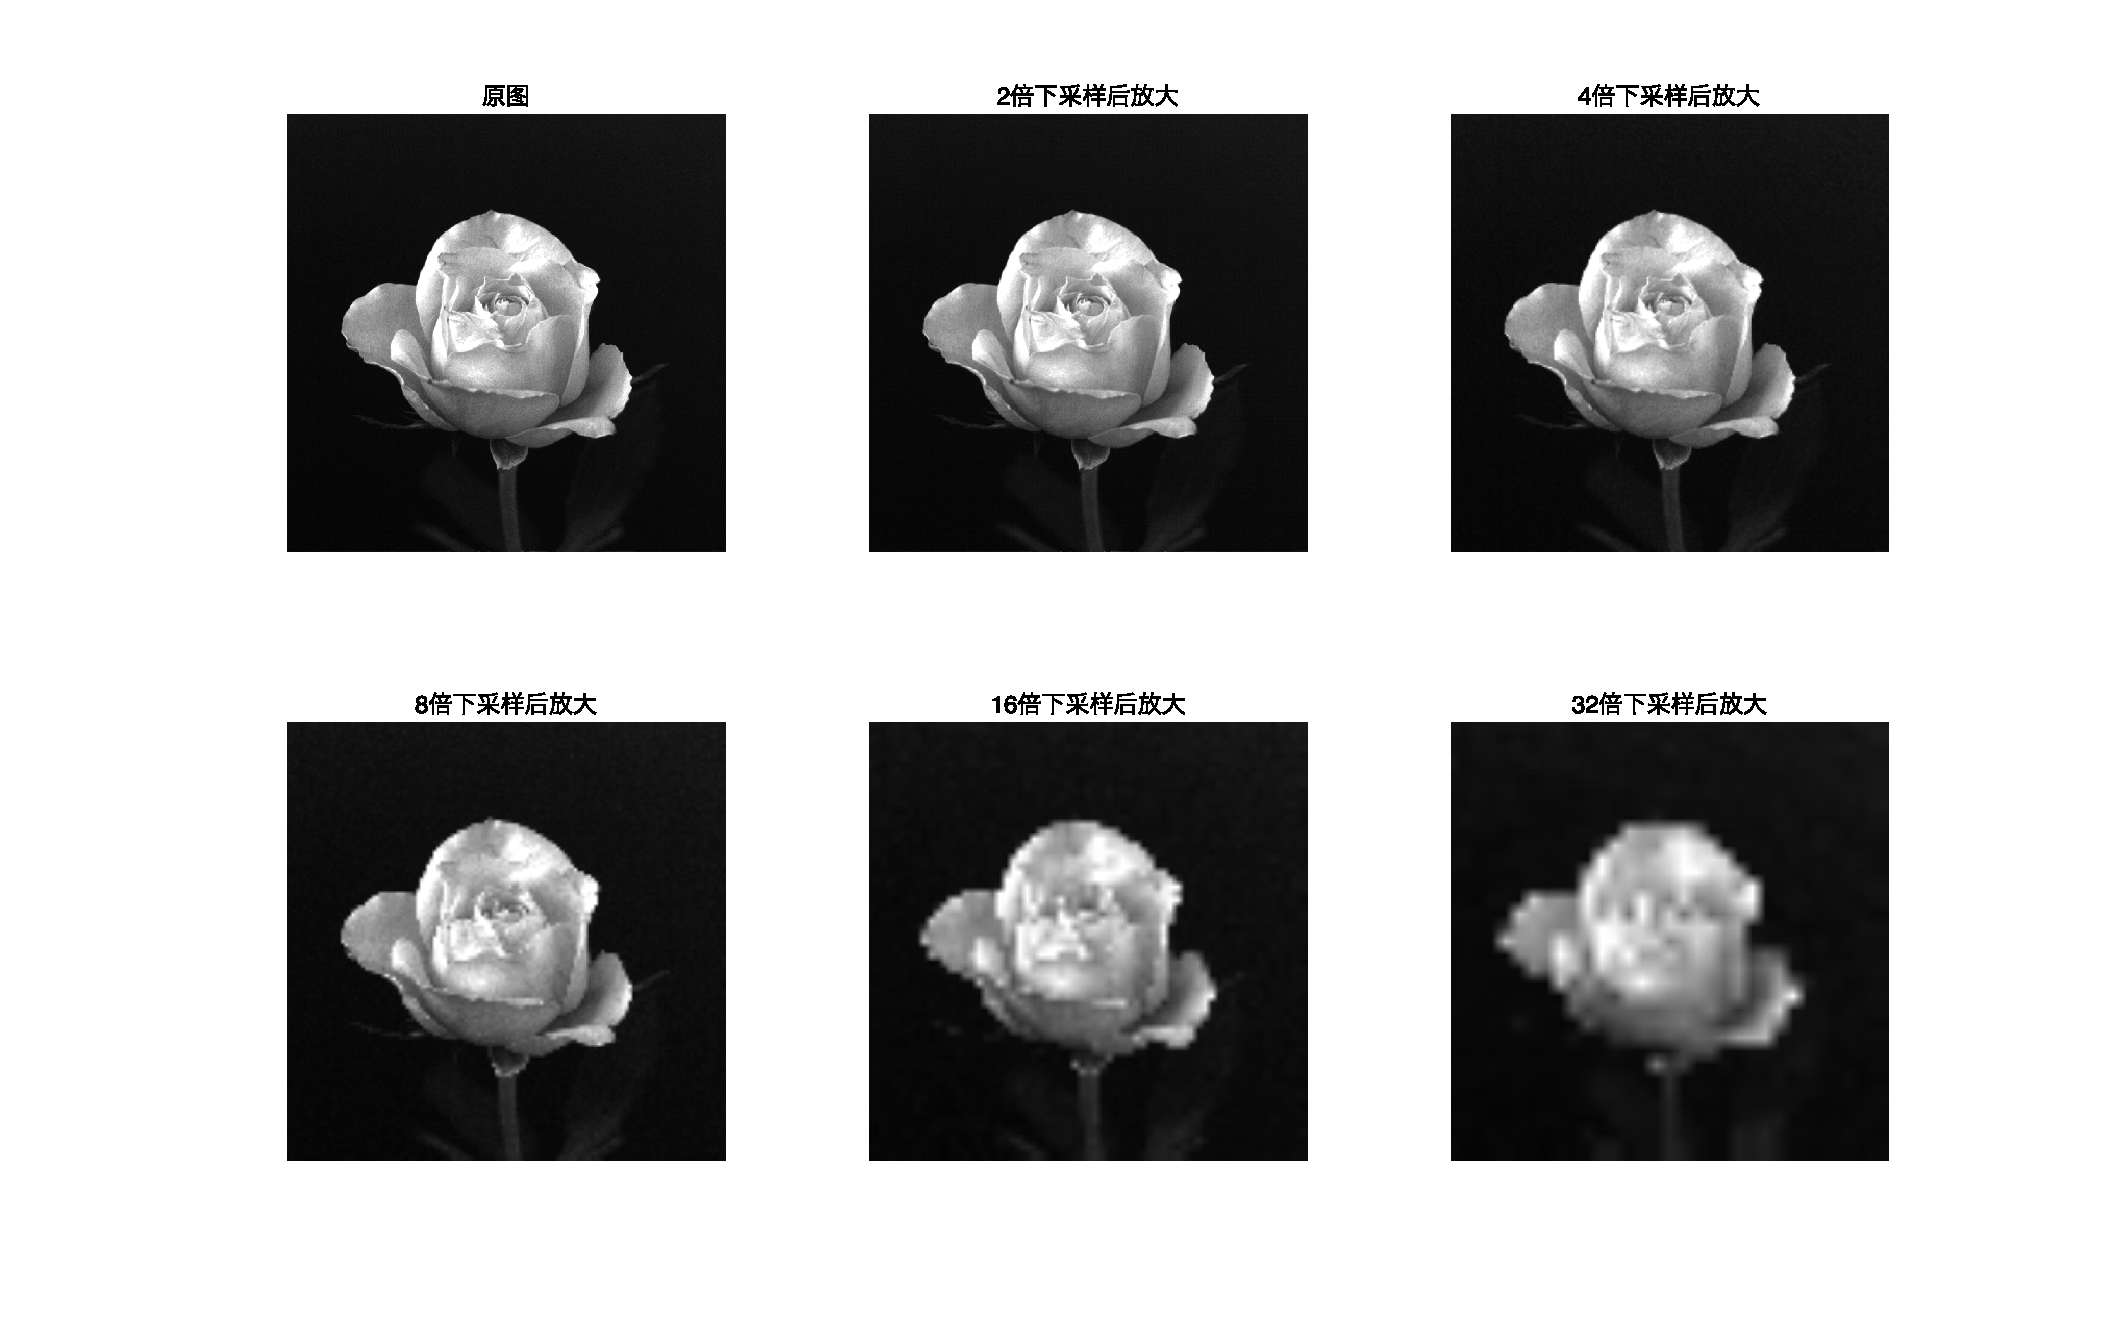
\includegraphics[width=1\textwidth,trim=20 20 20 20,clip]{images/sample_result.eps}
    \caption{采样后放大结果}
    \label{fig:sample}
\end{figure}

不同采样倍数得到图片的峰值信噪比如表\ref{tab:sample}所示。
\begin{table}[htbp]
    \centering
    \caption{不同情况下采样后放大与原图对比的PSNR值}
    \begin{tabular}{|c|c|c|c|c|c|}
   \hline 下采样倍数  & 2 & 4& 8 &16 & 32 \\
   \hline 自己实现  & 36.976&33.871 &30.075 &26.261 &22.863\\
   \hline matlab库函数 & 37.683&34.305 &30.415 &26.799 &23.354\\
   \hline
    \end{tabular}
    \label{tab:sample}
\end{table}

发现自己实现的采样和插值算法得到的实验结果与库函数实现的结果很接近,但从数值大小比较来看效果还有一点点差距。推测可能有两个方面的原因:一是下采样时采用的池化操作可能有所区别;二是在采样和插值时对图片边缘处的补全处理可能有所区别。

\subsection{任务二 \ 颜色空间的转换}
\subsubsection{H、S、I对图片质量的影响}
将RGB格式的彩色图片(iris.tif)转换为HSI格式。分别在H分量上加减0.2得到的结果如图\ref{fig:h}所示。分别在S分量上加减0.2得到的结果如图\ref{fig:s}所示。分别在I分量上加减0.2得到的结果如图\ref{fig:i}所示。
\begin{figure}[htb]
    \centering
    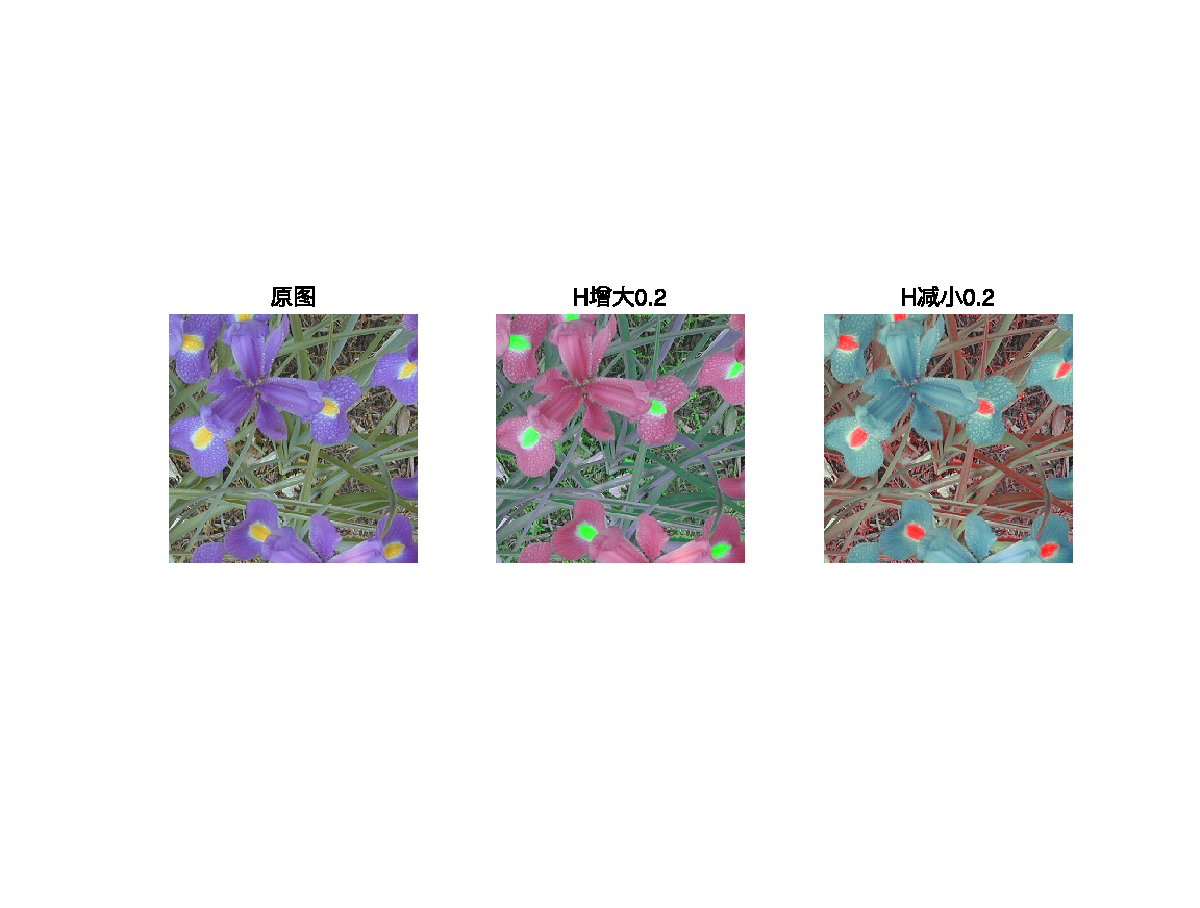
\includegraphics[width=0.9\textwidth,trim=50 150 50 130,clip]{images/H.eps}
    \caption{H分量对图片的影响}
    \label{fig:h}
\end{figure}
\begin{figure}[htbp]
    \centering
    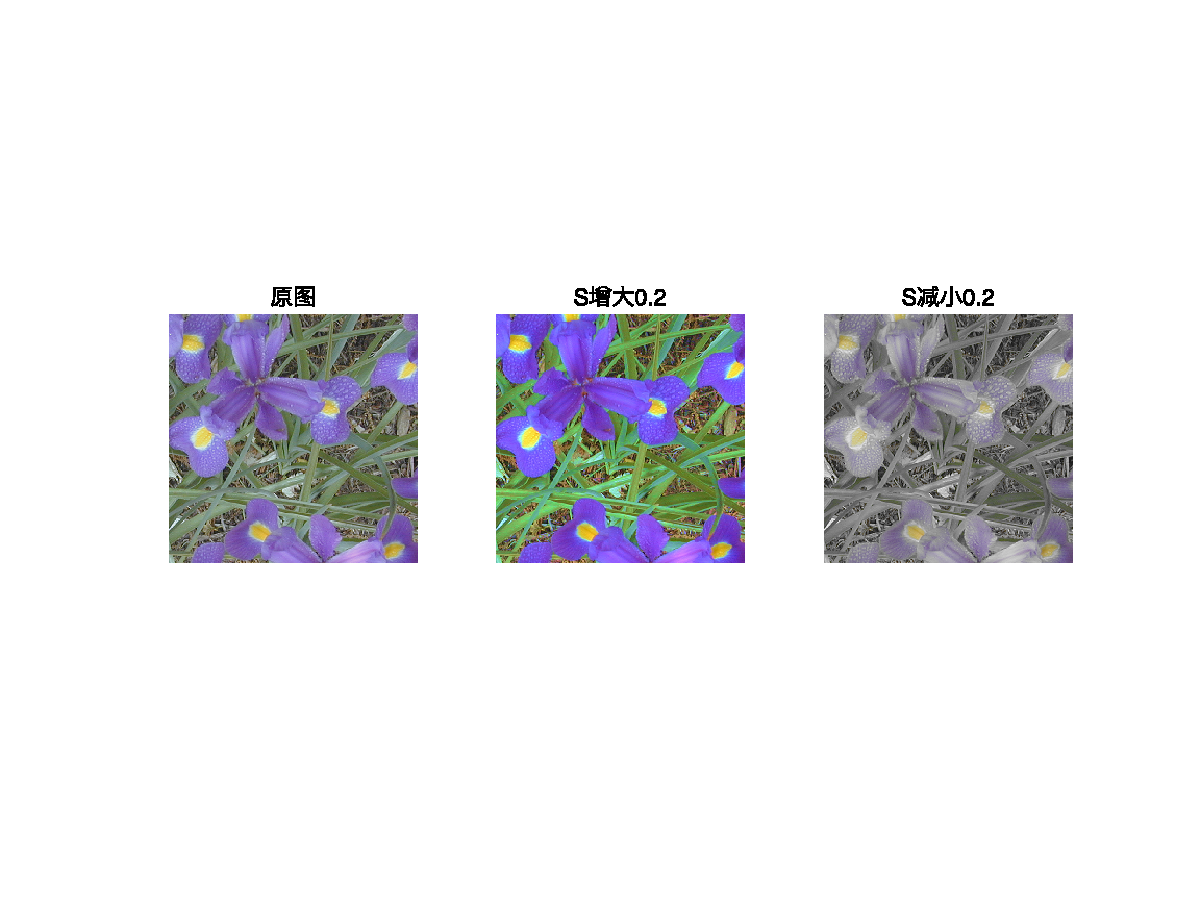
\includegraphics[width=0.9\textwidth,trim=50 150 50 130,clip]{images/S.eps}
    \caption{S分量对图片的影响}
    \label{fig:s}
\end{figure}
\begin{figure}[H]
    \centering
    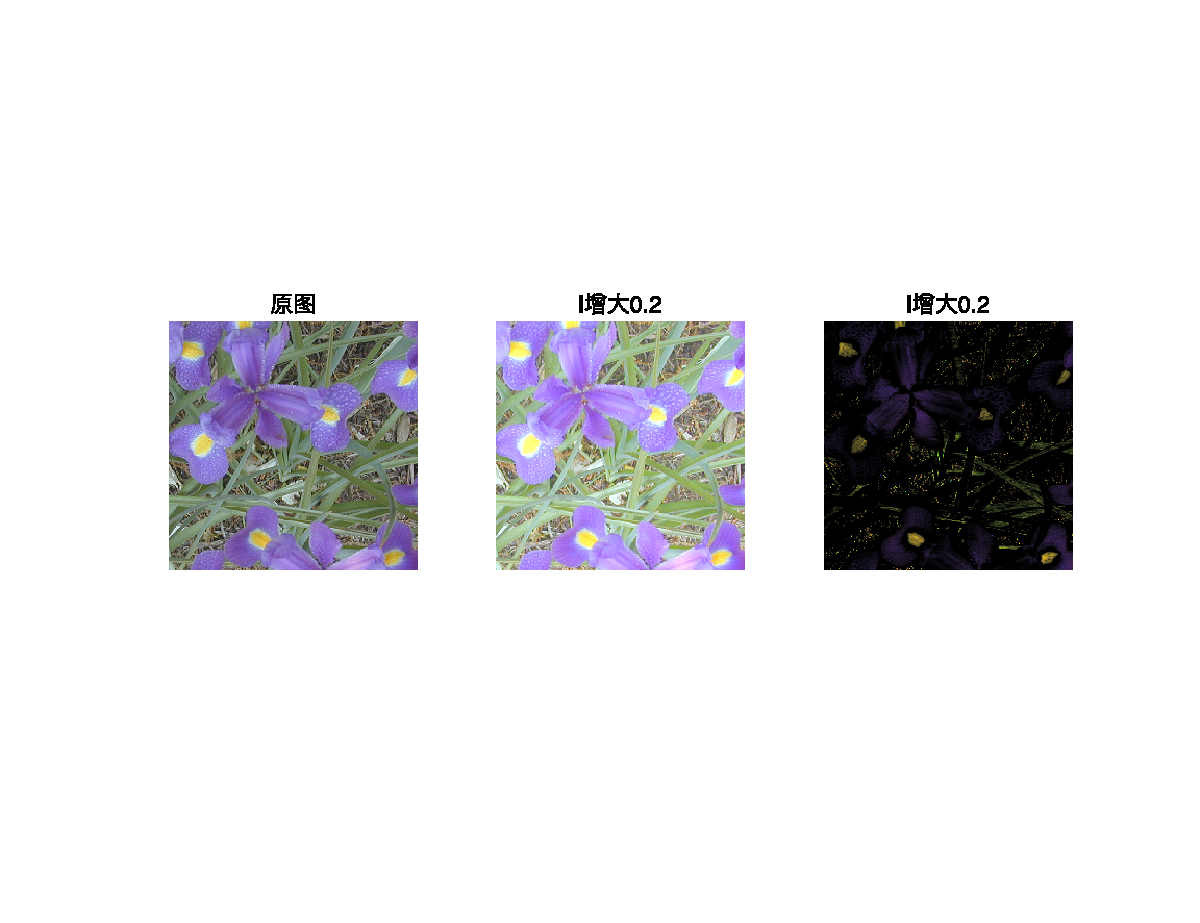
\includegraphics[width=0.9\textwidth,trim=50 150 50 130,clip]{images/I.eps}
    \caption{I分量对图片的影响}
    \label{fig:i}
\end{figure}

可以看到H分量代表图片的色调,H分量增大0.2时,紫色的花变成了红色;减少0.2时花变成了蓝色。S分量代表了颜色的饱和度,从实验结果可以看出,S越大,图片的饱和度越高。I分量可以代表图片的亮度,I增大0.2时,图片显著变亮;减小0.2时显著变暗,大部分区域变成接近黑色,但仍能观察到一些轮廓和颜色分布。
\subsubsection{Y、U、V对图片质量的影响}
将RGB格式的彩色图片(iris.tif)转换为YUV格式。分别在Y分量上加减50得到的结果如图\ref{fig:y}所示。分别在U分量上加减50得到的结果如图\ref{fig:u}所示。分别在V分量上加减50得到的结果如图\ref{fig:v}所示。
\begin{figure}[htb]
    \centering
    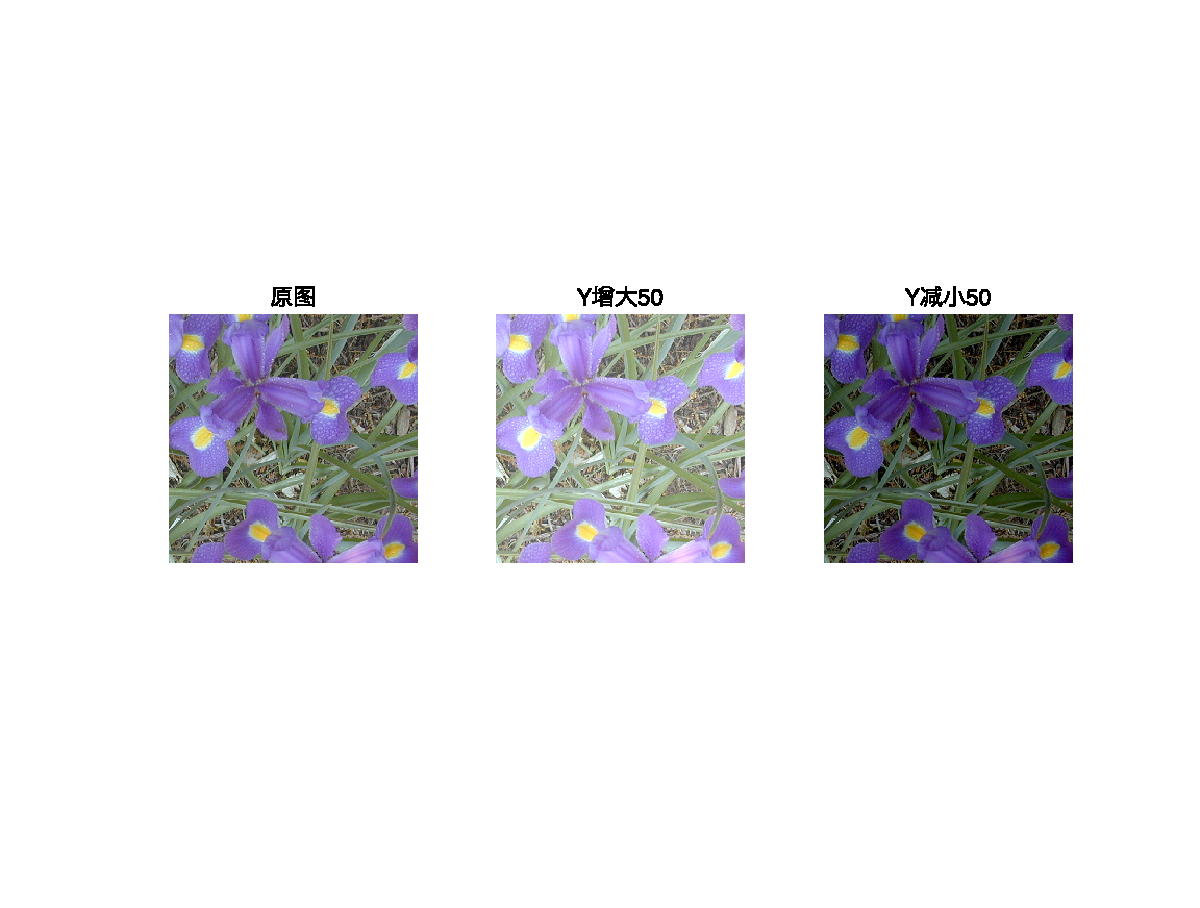
\includegraphics[width=0.9\textwidth,trim=50 150 50 130,clip]{images/Y.eps}
    \caption{Y分量对图片的影响}
    \label{fig:y}
\end{figure}
\begin{figure}[htbp]
    \centering
    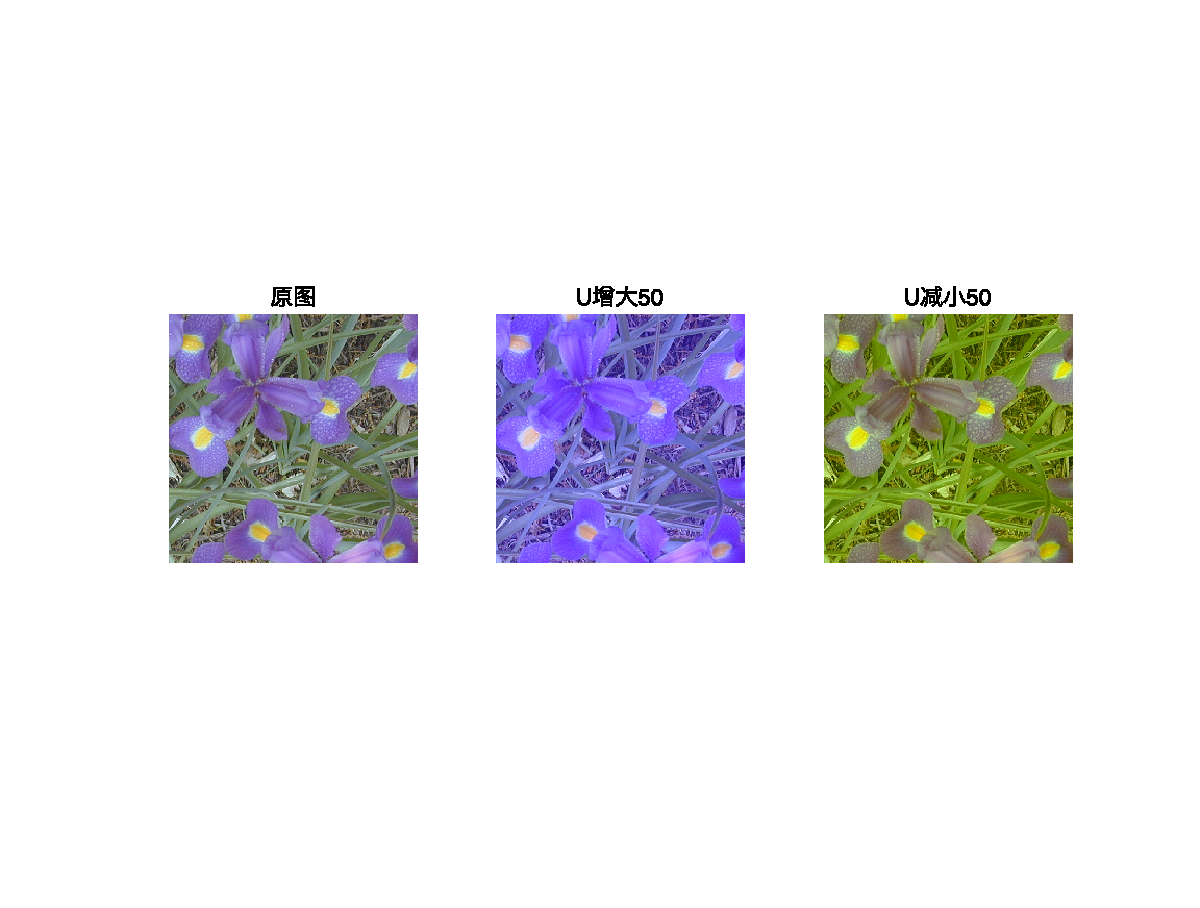
\includegraphics[width=0.9\textwidth,trim=50 150 50 130,clip]{images/U.eps}
    \caption{U分量对图片的影响}
    \label{fig:u}
\end{figure}
\begin{figure}[H]
    \centering
    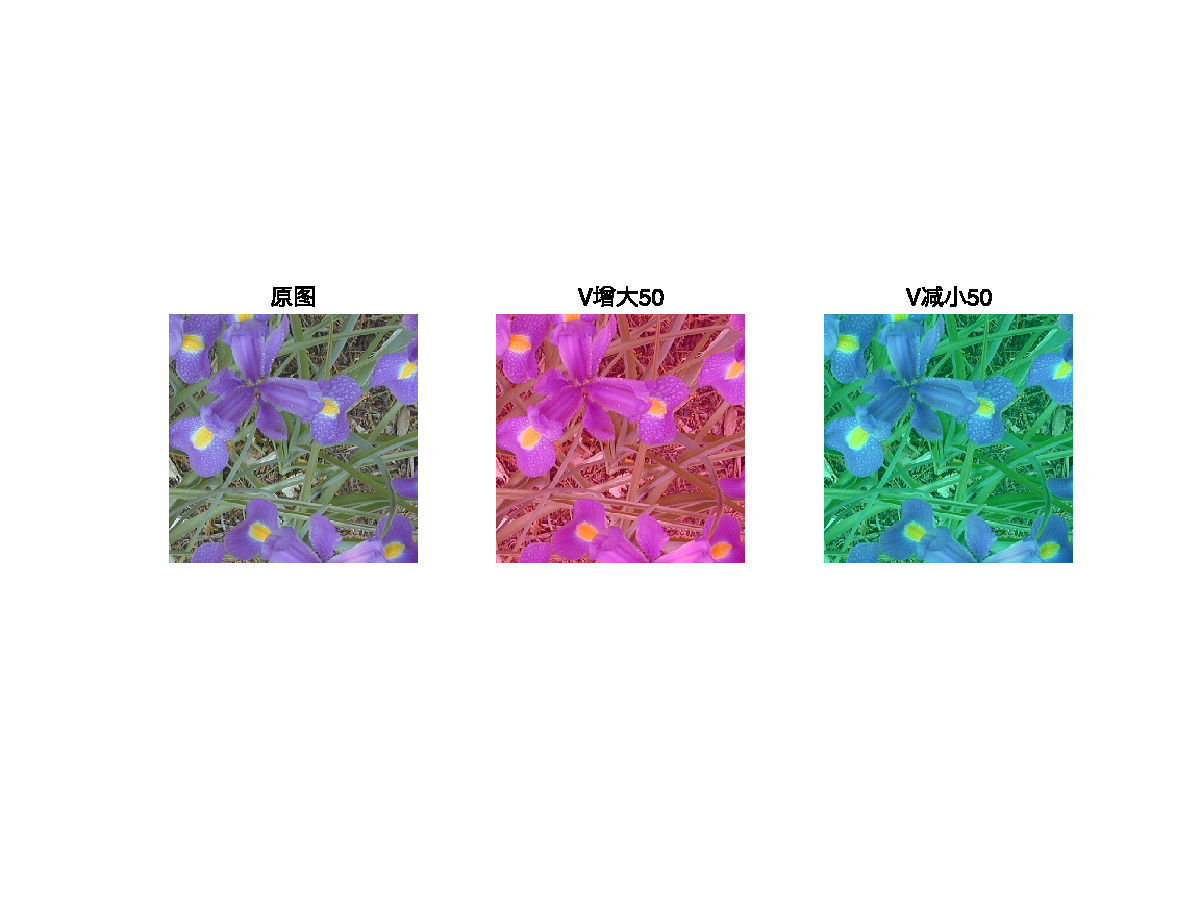
\includegraphics[width=0.9\textwidth,trim=50 150 50 130,clip]{images/V.eps}
    \caption{V分量对图片的影响}
    \label{fig:v}
\end{figure}

可以看到Y分量代表图片的色调,Y分量增大50时,图片显著变亮;减少50时图片显著变暗。U、V分量代表图片的色度,任一分量改变都会改变图片的整体色彩。在实验中我们对U、V分量的改变为一个常数50,主观效果类似于加上了一层颜色的滤镜。

\subsubsection{YUV采样格式对图片质量的影响}
主流采样格式有4:4:4、4:2:2和4:2:0,因为4:4:4相当于1倍采样与原图没有区别,这里测试了YUV4:2:2采样格式和4:2:0对图片PSNR值的影响,如表\ref{tab:yuv_psnr}所示。基于图片之间人眼几乎看不出差别,这里不浪费篇幅展示。
\begin{table}[hbtp]
    \centering
    \caption{不同YUV采样与插值方式的PSNR值}
    \begin{tabular}{|c|c|c|}
    
        \hline 采样格式 & 4:2:2 & 4:2:0 \\
        \hline 不插值 &35.137 & 33.833\\
        \hline 双线性插值 &39.781 &38.721 \\
        \hline
    \end{tabular}
    \label{tab:yuv_psnr}
\end{table}

可以看到,所有的PSNR值都大于33,在这个范围人眼很难分辨差别;4:2:2采样方式在相同插值操作下图像质量高于4:2:0;在相同的采样方式下,双线性插值对图片质量的提升效果显著。

\subsection{图片质量评价指标}
对于灰度图(lena.bmp),采用以下三种方式处理已达到$PSNR$值相同,主观效果不同,如图\ref{fig:standard}所示。四种方式得到的图片的$PSNR$和$SSIM$如表\ref{tab:standard} 所示。
\begin{enumerate}
    \item 图片整体灰度减小20
    \item 图片每个像素点加上高斯噪声(均值0,标准差20)
    \item 图片下采样到$33\times 33$后上采样到原尺寸($512\times 512$)(双三次插值)
\end{enumerate}
\begin{figure}[hbtp]
    \centering
    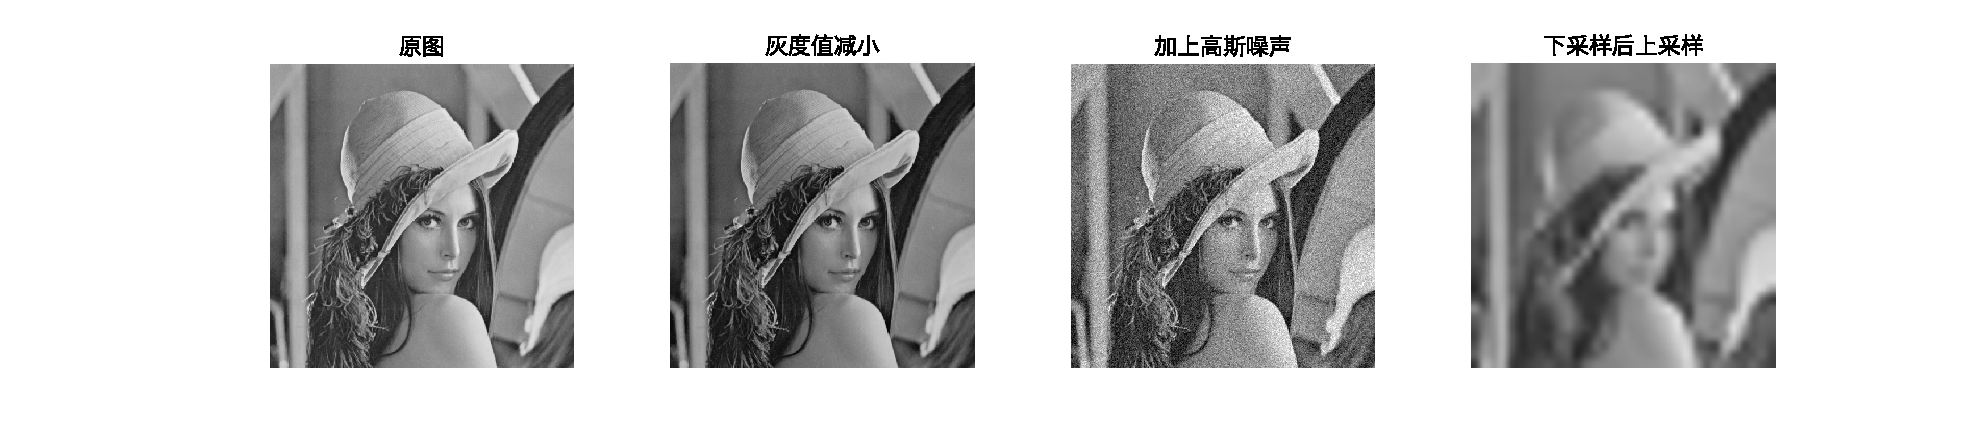
\includegraphics[width=1\textwidth,trim=50 20 50 0,clip]{images/standard.eps}
    \caption{不同处理方式得到的图片}
    \label{fig:standard}
\end{figure}
\begin{table}[hbtp]
    \centering
    \caption{不同处理方式得到的图片的PSNR和SSIM}
    \begin{tabular}{|c|c|c|c|}
        \hline 处理方式 & 灰度减小 & 加高斯噪声 & 下采样后上采样 \\
        \hline PSNR &22.1102 & 22.1099 &22.1851\\
        \hline SSIM &0.9687 &0.3400 & 0.6312 \\
        \hline
    \end{tabular}
    \label{tab:standard}
\end{table}

分析:
\begin{itemize}
    \item 三种处理方式$PSNR$值几乎一样。从定义也可以看出$PSNR$是纯粹比较每个像素点的大小后平均的结果。
    \item 从主观感受来看,灰度下降后图片细节依旧清晰,效果最好;加上高斯噪声后图片出现了很多噪点,但依然能很好地分辨出轮廓和颜色信息,效果次之;下采样后上采样后图片变得很模糊,效果最差。
    \item 三个图片的$SSIM$值差别很大。减小灰度的操作$SSIM$接近1,可以看出$SSIM$对图片整体的灰度或亮度变化不敏感;加上高斯噪声后$SSIM$变得很低,可以看出与图片信息无完全关的噪声对$SSIM$影响很大;因为$SSIM$计算过程中要进行加窗的平均操作,这个效果很类似与下采样的池化操作,所以下采样带来的模糊效果并不想对人眼那么不能接受。
\end{itemize}
\newpage
%--------致谢与说明-------
\section{致谢与说明}
本报告是上海交通大学电子工程系\textbf{EE229:数字图像处理}的课程作业报告。

感谢本课程老师周军老师的课堂讲授和指导,同时感谢即将批阅本报告的助教老师!






\end{document}

